% !TEX root = ../ausarbeitung.tex

\chapter{Diskussion} %TODO Ref!!!
\label{chap:discussion}
In diesem Kapitel sollen die Ergebnisse des Nutzertests interpretiert werden. Durch die sehr kleine Stichprobenzahl ist es nicht möglich statistische Erhebungen durchzuführen, allerdings können Tendenzen aus den gewonnenen Daten abgelesen werden. 
\section{Challenge}
\label{sec:challengeDisk}
Wie man im Boxplot zur Challenge erkennen kann, lag der Durchschnitt der Challengebewertungen in der TopDown Perspektive höher als in der ThirdPerson Perspektive. Dies könnte daran liegen, da es in der TopDown Perspektive schwieriger war die Schlange zu erkennen, da die Schlange und der Boden eine ähnliche Farbe haben. In der ThirdPerson Perspektive war die Schlange leichter erkennbar, da die Kamera sehr nah an der Schlange war. Durch diese Perspektive musste man teilweise nicht Schlangen-Grün von Umgebungs-Grün unterscheiden, da der Himmel in dieser Perspektive auch sichtbar war. Ein Vergleich hierzu sieht man in folgender Grafik.

%TODO Vielleicht Bild hier hin von Perspektiven?

\section{Competence}
\label{sec:competenceDisk}
In dieser Kategorie wurde abgefragt wie erfolgreich sich die Spieler während des Spielens gefühlt haben. Anhand des Boxplots ist hier zu erkennen, dass es in der TopDown Ansicht größere Schwankungen gab. Auf diesen Wert kann der Kontrast der Schlange auch Einfluss genommen haben, da sich die Spieler weniger erfolgreich fühlen wenn sie die Schlange nicht genau erkennen konnten. Der Median liegt hier aber im oberen Bereich. Dies kann daran liegen, dass Spieler, die zuerst die Third Person Perspektive gespielt haben einen leichteren Umstieg auf die TopDown Version hatten. Das Spielprinzip war zu dieser Zeit bereits klar sowie welche Art von Character man im Spiel steuert. Insgesamt muss man aber sagen, zeigt die ThirdPerson Perspektive bessere Tendenzen, da hier die Competence-Werte enger beieinander liegen.
\section{Flow}
\label{sec:flowDisk}
Der Boxplot zu den Flow-Werten zeigt uns, dass tendenziell die ThirdPerson Perspektive den Spieler mehr eingenommen hat. Dies kann darin begründet sein, dass man in dieser Perspektive eher das Sichtfeld des zu steuernden Characters sieht als in der TopDown Perspektive. Ein weiterer Grund hierfür kann sein, dass der Spieler sich hier mehr auf das Spiel konzentrieren muss, da er nicht direkt alle Zahlen im Überblick hat. In der TopDown Perspektive sieht der Spieler direkt alle Äpfel mit deren Zahlen und kann sich leicht einen Plan zurecht legen. In der ThirdPerson Perspektive sieht dies anders aus. Hier muss der Spieler sich erst über das Spielfeld bewegen um ein Paar Äpfel zu finden, welches zusammen addiert die gesuchte Zahl ergibt. Dies wird außerdem dadurch erschwert, da die Zahlen sich nicht zum Spieler drehen und damit immer optimal angezeigt werden. Der Spieler muss also auch umgedrehte Zahlen lesen können. Dies alles deutet darauf hin, dass der Spieler sich in der ThirdPerson Variante mehr auf das Spiel fokusieren muss. 
\section{Immersion}
\label{sec:immersionDisk}
Auch der Immersions-Wert der ThirdPerson Variante deuted darauf hin, dass diese Version den Spielern besser gefallen hat. Dies kann dadurch begründet sein, dass man in der TopDown Perspektive relativ schnell alles gesehen hat, während man in der ThirdPerson Perspektive die Umgebung erst erkunden kann und mehr Details der Umgebung sehen kann als in der TopDown Perspektive.
\section{Negative Effect}
\label{sec:negeffDisk}
In dieser Kategorie zeigen beide Spiele eher die Tendenz zu keinen negativen Effekten. Bei der ThirdPerson Variante kann der sehr geringe Wert über 0 daher kommen, dass in der zu spielenden Version ein kleiner Kamera Fehler war, der nach dem Ende einer Spielrunde kurz ein verzerrtes Bild vom Spiel angezeigt hat. In der TopDown Version gibt es einen großen Wert über den 1.5 . Dieser ist während der Ausführung des Nutzertests auch aufgefallen und war von einem Kind, dass die Entscheidung damit begründet hat lieber wieder die andere Version spielen zu wollen, da es Third Person zuerst gespielt hat. Man kann also erkennen, dass die Negativen Effekte für beide Versionen gegen 0 gehen.
\section{Positive Effect}
\label{sec:poseffDisk}
Die Werte für die Positiven Effekte während des Spielens sind für beide Versionen etwa im gleichen Bereich mit um die 2.6 bis 3.5. Mit einer größeren Anzahl an Nutzertests kann man hier vielleicht einen signifikanteren Unterschied erkennen. Beide Versionen weisen aber die Tendenz auf eher viele positive Effekte herforgerufen zu haben.
\section{Tension}
\label{sec:tensionDisk}
In dieser Kategorie hat sich vor allem während des Nutzertests die Frage 18 als sehr interessant heraus gestellt.
\begin{quote}
Ich habe beim Spielen gemotzt
\end{quote}
Der Boxplot zeigt uns hier, dass man im Schnitt in der TopDown Variante mehr Probleme hatte. Dies kann wieder ,wie bereits in Challenge erwähnt, daran liegen, dass die Schlange nicht gut erkennbar war. Hier haben die Kinder aber auch viel Anhand der Steuerung gemeckert. Wenn die Schlange im TopDown Modus sich von unten nach oben bewegt ist es ganz klar, dass beim drücken auf die rechte Pfeiltaste sich die Schlange nach rechts bewegt und beim drücken auf die linke Pfeiltaste sich die Schlange nach links bewegt. Dies trifft allerdings nicht mehr zu, wenn die Schlange sich gerade von oben nach unten bewegt. Dieser Umstand hat den meisten Kindern hier Probleme bereitet und wird in \ref{fig:controlIssue} nochmals grafisch dargestellt. Wenn die Pfeiltaste nach rechts durchgehend gedrückt gehalten wird, würde man zunächst das linke Bild sehen und anschließend das rechte Bild.
\begin{figure}[htb]
	\centering
	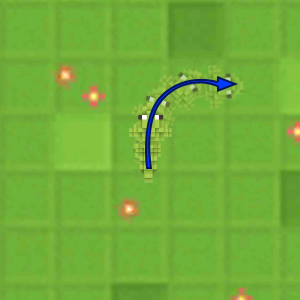
\includegraphics[width=0.3\textwidth]{SnakeDirection1}
	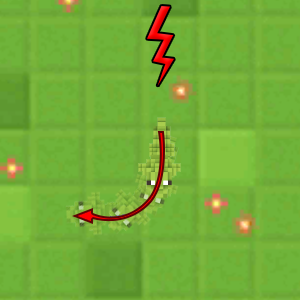
\includegraphics[width=0.3\textwidth]{SnakeDirection2}
	\caption{Links: Pfeiltaste nach rechts = nach rechts bewegen. Rechts: Pfeiltaste nach rechts = nach links bewegen\label{fig:controlIssue}}
\end{figure}
\section{Startpunktzahl}
\label{sec:startpointsDisk}
Am Anfang hatte jeder Spieler direkt 10 Punkte ohne einen Apfel gegessen zu haben, dies hätte eigentlich nicht der Fall sein sollen, hat aber Interessante Beobachtungen eingebracht. Viele der Kinder scheinen nicht bemerkt zu haben, dass sie direkt mit 10 Punkten starten und gingen davon aus, dass sie schon etwas geschafft haben. Wenn die Kinder direkt am Anfang die Schlange sich selbst fressen ließen, sahen sie trotzdem glücklich mit den zumindest 10 Punkten aus.
\section{Ausblick}
\label{sec:ausblickDisk}
In diesem Kapitel sollen die Erweiterungsmöglichkeiten des Spiels sowie mögliche weitere Studien disskutiert werden.
\subsection{Ausblick in Spielerweiterungen}
Das Spiel MathSmashers lässt sich noch in vielen Bereichen verbessern. Wie bereits in \ref{sec:negeffDisk} erwähnt wäre interessant zu sehen ob es hier zu keinen negativen Effekten mehr kommt, wenn der Kamerafehler im Spiel beseitigt wurde. Auch sonst sind viele Verbesserungen im Design und den Visuellen Effekten möglich. Einer der wichtigsten Punkte hier wird für die TopDown Version der Kontrast der Schlange sein. Dieser wurde mehrheitlich unter den Nutzern als verbesserungswürdig eingestuft. Da in dem verwendeten Asseet-Pack mehrere Schlangendesigns enthalten sind, könnte man hier am Anfang des Spiels den Spieler seine Schlange wählen lassen. Dies könnte den Effekt haben, dass der Spieler sich auch gleichzeitig mehr mit seiner Spielfigur identifizieren kann und somit der Flow-Wert steigen würde. Für einen vielleicht steigenden Immersions-Wert könnte zusätzlich sorgen, wenn man die Grafik für den Boden überarbeitet, damit diese ebenso scharf dargestellt wird wie der Rest der Spielwelt.\\
\\
Auch für einen höheren Challenge-Wert kann das Spiel optimiert werden. So wäre es zum Beispiel möglich das Spiel auch für höhere Klassenstufen noch interessant zu machen. Der Anstieg der Schwierigkeitsstufe auf ein Level mit verfaulenden Äpfeln wurde für diesen Nutzertest so weit nach oben gesetzt, dass kein Spieler zu diesem Level kam. Das war für diese Altersgruppe aber auch nicht vorgesehen. Man kann also in neueren Versionen das Levelsystem anpassen um auch zu diesem Level nach einer angemessenen Spielzeit zu kommen. Auch mögliche Erweiterungen des Levelsystems wurden festgehalten. So ist es möglich weitere Level einzufügen in denen zum Beispiel 'Fake-Äpfel' auftauchen. Dies sind Äpfel, die dem Spieler effektiv nicht helfen die gesuchte Zahl zu bilden. Das heißt sie sollten von dem Spieler nicht gegessen werden. Damit sind auch weitere Erweiterungen möglich, die die Schlange fressen kann. So ist es dann auch möglich ein Item einzuführen, welches diese 'Fake-Äpfel' identifizieren kann oder andere Eigenschaften mit sich bringt, wie Items die die Schlange verkürzen oder verlangsamen, aber auch Items mit denen der Spieler die zu suchende Zahl ändern kann als eine Art Joker.
\subsection{Ausblick auf weitere Nutzertests}
Zunächst ist ein Nutzertest mit einer größeren Stichprobenmenge sinnvoll, aber auch weitere Fragen können durch Nutzertests beantwortet werden. So zum Beispiel ob Startpunkte, wie in \ref{sec:startpointsDisk} beschrieben, den Wert der positiven Effekte steigert oder unerheblich für diesen ist. Außerdem wurde wie in \ref{sec:tensionDisk} beschrieben ein Problem mit der Steuerung der TopDown Variante festgestellt. Hier ist über Nutzertests zu überprüfen ob eine Änderung der Steuerung zur klassischen Snake Variante sinnvoll wäre. Im klassischen Snake steuert man die Schlange mit allen Richtungstasten und gibt jeweils an in welche Richtung sich die Schlange bewegen soll. Dabei sind ausschließlich $90^\circ$ Drehungen möglich.
\section{Zusammenfassung}
\label{sec:conclusionDisk}
In Bezug auf die Zielsetzung dieser Arbeit, welche Variante des Spiels den Nutzern besser gefallen hat, gab es auch weitere schriftliche Fragen. Diese bestätigen die durch den GEQ bezogenen Tendenzen, dass die ThirdPerson Perspektive den Nutzern mehr Spaß bereitet hat. Alle Nutzer haben bei der Frage welches Spiel ihnen mehr Spaß gemacht hat die ThirdPerson Variante angegeben. Dem entsprechend wurde auch bei allen Nutzern die TopDown Variante als schwieriger gewertet. Diese Schwierigkeiten hatten auch Auswirkungen auf die Kategorien des GEQ, wie bereits in den einzelnen Kapiteln beschrieben.\\
Insgesamt können beide Forschungsfragen, aufgrund der geringen Nutzertest-Teilnehmer, nicht eindeutig beantwortet werden. Allerdings können wir anhand der Tendenzen sagen, dass ein solches Lernspiel zur Unterstützung der Addition über Partnerzahlen den Kindern mit hoher Wahrscheinlichkeit Spaß bereitet. Außerdem konnte eine starke Tendenz zur ThirdPerson Variante erkannt werden. Ob diese nach Behebung einiger Schwierigkeiten der TopDown Perspektive bestehen bleibt, ist durch zukünftige Tests zu ermitteln.